% !TeX spellcheck = it_IT
\newpage
\section{Equazioni non lineari}
Stiamo considerando equazioni del tipo $f(x)=0$ dove la funzione $f$ non è lineare (quindi non è una retta). Di fronte a questo tipo di equazioni, ci sono due difficoltà:
\begin{itemize}
	\item Non c'è una teoria generale sul \textit{numero} e sull'\textit{esistenza} delle \textbf{soluzioni}
	\item Non esistono metodi diretti di risoluzione
\end{itemize}

\begin{example}
	Determinare il numero di soluzioni reali dell'equazione
	\begin{equation*}
		f(x)=x \log x -1 = 0
	\end{equation*}
	Il primo passo è tracciare un grafico approssimativo di questa funzione:
	\begin{itemize}
		\item \textbf{Dominio}: $x>0$
		\item \textbf{Limiti}:
		\begin{align*}
			& \lim_{x \to + \infty} x \log x -1 = + \infty \\
			& \lim_{x \to 0^+} x \log x = \lim_{x \to 0^+} \frac{log x}{\frac{1}{x}} = \lim_{x \to 0^+} \frac{\frac{1}{x}}{-\frac{1}{x^2}} = \lim_{x \to 0^+} - \frac{x^2}{x} = 0 \Longrightarrow \lim_{x \to 0^+} x log x -1 = -1 
		\end{align*}
		\item \textbf{Derivata prima}: \begin{align*}
			& f'(x) = \log x + x \cdot \frac{1}{x} = \log x + 1 \\
			& f'(x) \geq 0 \Leftrightarrow log x + 1 \geq 0 \Leftrightarrow log x \geq -1 \Leftrightarrow x \geq \frac{1}{e}
		\end{align*}
		\item \textbf{Derivata seconda}: $f''(x)=\frac{1}{x} \geq 0 \quad \forall x > 0$
	\end{itemize}
	\begin{center}
		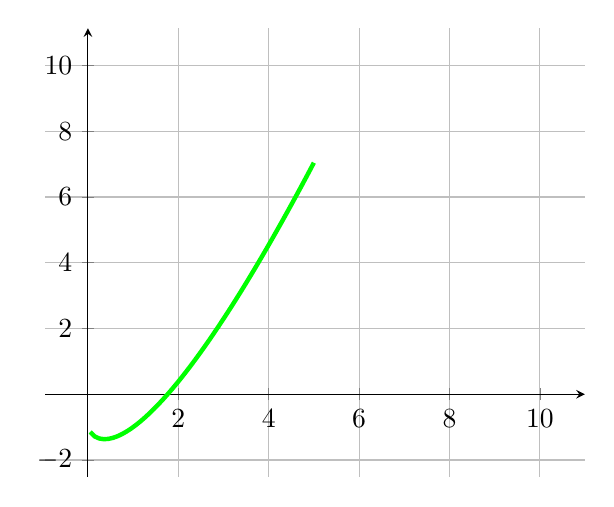
\begin{tikzpicture}
			\begin{axis}[grid=both,
				xmax=10,ymax=10,
				axis lines=middle,
				samples=100,
				enlargelimits]
				\addplot[green, ultra thick]  {x*ln(x)-1};
			\end{axis}
		\end{tikzpicture}
	\end{center}
	Quindi possiamo dire che 
	\begin{equation*}
		\exists ! \alpha \in \mathbb{R} \vert f(\alpha) = 0
	\end{equation*}
	Ci serve dare un \textbf{intervallo di localizzazione} della soluzione, ad esempio:
	\begin{align*}
		& f(1) = -1 \\
		& f(2) = 2 \log 2 -1 = log 4 -1 \\
		& \Rightarrow \alpha \in [1,2]
	\end{align*}
\end{example}

\subsection{Tecnica della separazione}
A partire da una funzione complessa, mi riconduco a funzioni più semplici e vedo dove si intercettano.
\begin{example}
	Supponiamo di avere
	\begin{equation*}
		x \log x -1 = 0 \Leftrightarrow x \log x = 1 \Leftrightarrow \log x = \frac{1}{x}
	\end{equation*}
	Che sul grafico sono
	\begin{center}
		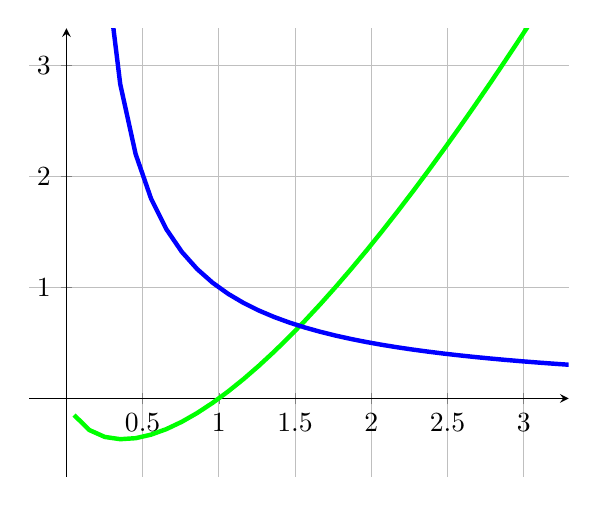
\begin{tikzpicture}
			\begin{axis}[grid=both,
				xmax=3,ymax=3,
				axis lines=middle,
				restrict x to domain=0:4,
				restrict y to domain=-2:4,
				samples=100,
				enlargelimits]
				\addplot[green, ultra thick]  {x*ln(x)};
				\addplot [blue, ultra thick] {1/x};
			\end{axis}
		\end{tikzpicture}
	\end{center}
\end{example}

\begin{example}
	Data la seguente funzione
	\begin{equation*}
		f(x) = e^x - 2x = 0 \Leftrightarrow e^x = 2x
	\end{equation*}
	È difficile usare il metodo della separazione perché l'intersezione non è facile da trovare. \\
	Usiamo quindi la soluzione grafica:
	\begin{itemize}
		\item \textbf{Dominio}: $\forall x \in \mathbb{R}$ che possiamo scrivere anche come $C^\infty (\mathbb{R})$
		\item \textbf{Limiti}:
		\begin{align*}
			& \lim_{x \to + \infty} e^x -2x = \lim_{x \to + \infty} e^x (1 - \frac{2x}{e^x}) = 0\\
			& \lim_{x \to - \infty} e^x -2x = + \infty\\
		\end{align*}
		\item \textbf{Derivata prima}: \begin{align*}
			& f'(x) = e^x -2 \\
			& f'(x) \geq 0 \Leftrightarrow e^x \geq 2 \Leftrightarrow x \geq \log 2
		\end{align*}
		\item \textbf{Derivata seconda}: $f''(x)=e^x$
	\end{itemize}
	\begin{center}
		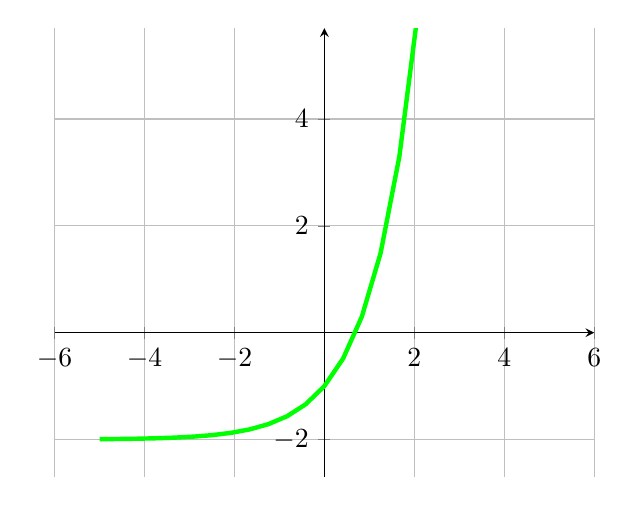
\begin{tikzpicture}
			\begin{axis}[grid=both,
				xmax=5,ymax=5,
				axis lines=middle,
				enlargelimits]
				\addplot[green, ultra thick]  {pow(e,x)-2};
			\end{axis}
		\end{tikzpicture}
	\end{center}	
	Calcoliamo adesso il valore in $\log 2$:
	\begin{equation*}
		f(\log 2) = e^{\log 2} - 2 \log 2 = 2-2 \log 2 = 2 (1-\log 2)
	\end{equation*}
\end{example}

\begin{example}
	Data la funzione:
	\begin{equation}
		f(x)= x^3 -6x +1 = 0
	\end{equation}
	In questo esempio abbiamo un polinomio e abbiamo quindi un'\textbf{equazione algebrica} di terzo grado. Quindi sappiamo il numero di soluzioni \textit{complesse}, nel nostro caso $3$. A noi però interessa il numero di soluzioni reali. Sapendo che quelle complesse devono andare sempre in coppia, potremo avere o due soluzioni complesse e una reale oppure tre soluzioni reali. Studiamo la funzione:
	\begin{itemize}
		\item \textbf{Dominio}: $\forall x \in \mathbb{R}$
		\item \textbf{Limiti}:
		\begin{align*}
			& \lim_{x \to + \infty} x^3 -6x +1 = + \infty\\
			& \lim_{x \to - \infty} x^3 -6x +1 = - \infty\\
		\end{align*}
		Sappiamo quindi che esiste sicuramente almeno un punto in cui la funzione vale $0$ per il teorema dell'esistenza degli zeri.
		\item \textbf{Derivata prima}: \begin{align*}
			& f'(x) = 3x^2-6 \\
			& f'(x) = 0 \Leftrightarrow x^2 = 2 \Leftrightarrow x = \pm \sqrt{2} \to x < -\sqrt{2} \land x > \sqrt{2}
		\end{align*}
		\item \textbf{Derivata seconda}: $f''(x)=6x \to f''(x) > 0 \Leftrightarrow x>0$
	\end{itemize}
	\begin{center}
		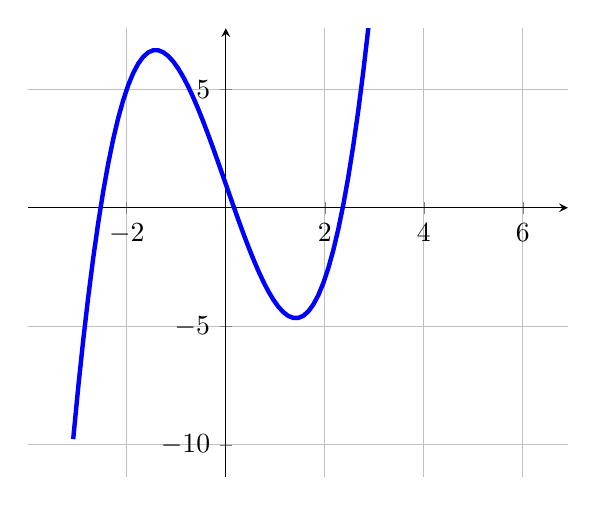
\begin{tikzpicture}
			\begin{axis}[grid=both,
				xmax=6,ymax=6,
				axis lines=middle,
				restrict x to domain=-4:4,
				restrict y to domain=-10:10,
				samples=100,
				enlargelimits]
				\addplot[blue, ultra thick] (x,x^3-6*x+1);
			\end{axis}
		\end{tikzpicture}
	\end{center}
	Quindi ci sono tre soluzioni reali, che possiamo localizzare come:
	\begin{align*}
		& \beta \in [0, \sqrt{2}]\\
		& \gamma \in [\sqrt{2}, 3]\\
		& \alpha \in [-3,-2]
	\end{align*}
\end{example}
